
\section{Materials and methods}

\subsection{Neurogenetic methods used for estimating ring neuron receptive fields}\todo{new section added}
\label{sec:methods:seelig}
In this section I shall briefly outline the method employed in \citeA{Seelig2013} to acquire the visual receptive fields used as a basis for the modelling in this chapter (as well as Chapter~\ref{ch:drosonavigation}).

The goal of Seelig and Jayaraman's \cite{Seelig2013} work was to examine responses of lateral triangle microglomeruli (the ring neurons) to visual stimuli.
For this, they employed two-photon calcium imaging to examine the activity of genetically targeted subsets of microglomeruli, the R2 and R3/R4d neurons.
Fluorescence was recorded for head-fixed flies held in an arena with a curved display composed of an LED array.
In order to map the receptive fields, the flies were presented with a series of flashing dots at random locations on the visual display; the fine structure of the receptive fields was then revealed by using white-noise stimuli \cite<see, e.g.,>{Weber2010}.
The accuracy of the estimated receptive fields was then verified by correlating predicted with actual responses to novel bar stimuli (and a high degree of correspondence, was found).
The orientation tuning for the different receptive fields was estimated by presenting the flies with a series of vertical bar stimuli (bright on a dark background) at different elevations, which moved across the display horizontally (in each direction).

\subsection{Turning visual receptive field data into visual filters}
\label{sec:methods:preprocessing}
The RFs used in these simulations were based on the data presented in \citeA{Seelig2013}.
We first extract the image representations of the RFs from the figure (Extended Data Figure 8); this gives us images of $112\times 252$ pixels for R2 neurons and $88\times 198$ pixels for R4d.
Given the visual field is taken as $120\degree\times 270\degree$, this corresponds to a resolution of 1.07\degree\ and 1.36\degree\ per pixel, respectively.
As data is given for multiple flies, we averaged the RFs for the different glomeruli across flies ($2\le N(\mathrm{R2}) \le 6, 4\le N(\mathrm{R4})\le 7$). This process is summarised in Figure~\ref{fig:avkernels}. Each point on the image was assigned a value ranging from --1 for maximum inhibition to 1 for maximum excitation, based on the values given by the colour scale bars in \citeA{Seelig2013}.
These images were then thresholded to give a kernel $g(i,j)$:
$$
g(i,j) = \left\{ \begin{array}{rl}
		   1 & \mbox{for } R_{i,j} \ge T; \\
                  -1 & \mbox{for } R_{i,j} \le -T; \\
                   0 & \mbox{otherwise.}
                  \end{array}
          \right.
$$
where $g(i,j)$ is the ($i,j$)th pixel of the kernel, $R_{i,j}$ is the ($i,j$)th value of the processed receptive field image and $T$ is the threshold value, here $0.25$ (Figure~\ref{fig:avkernels}A).

We took the centroid of the largest excitatory region as the `centre' of each of the kernels.
The excitatory regions were then extracted using \Matlab's \texttt{bwlabeln} function (with eight-connectivity) and the centroid, $(x,y)$, with the \texttt{regionprops} function.
The mean centroid, $(\bar{x},\bar{y})$, across flies is then calculated and the kernels are recentred on this point:
$$
\hat{g}(i,j) = \left\{ \begin{array}{ll} g(i+y-\bar{y},j+x-\bar{x}) & \mbox{for } 1\le i+y-\bar{y}\le m \mbox{ and } 1\le j+x-\bar{x}\le n;\\
0 & \mbox{otherwise.} \end{array} \right.
$$
where $\hat{g}(i,j)$ is the recentred kernel (Figure~\ref{fig:avkernels}C).

We next calculate the average kernel across flies, $\bar{g}(i,j)$, and threshold again:
\begin{align*}
\bar{g}(i,j) &= \left\{ \begin{array}{rl}
			-1 & \mbox{for } c \le -T; \\
			 1 & \mbox{for } c \ge T; \\
			 0 & \mbox{otherwise.} 
			\end{array} \right. \\
\mbox{where } c &= \frac{1}{|\mathbf{G}|}\sum\limits_{\hat{g} \in \mathbf{G}} \hat{g}(i,j)
\end{align*}
where $\mathbf{G}$ is the set of kernels being averaged and $T$ is the threshold (again: 0.25). Note that instead of thresholding then averaging the raw images, $R$, before thresholding them again, we could have averaged the raw pixel values. The reason we did not do so was to reduce noise on the raw images; tests showed a negligible difference in performance when doing the latter.

In order to calculate the activation for a given RF on presentation of an image the RF must first be resized to the same size as the image.
This is accomplished by resizing the average RF, $\bar{g}(i,j)$ (using \Matlab's \texttt{imresize} function with appropriate normalisation).
Finally, the kernel is rethresholded and the excitatory and inhibitory regions are assigned different values:
$$
K_{i,j} = \left\{
\begin{array}{rl}
\frac{1}{N_\mathrm{exc}}, & \mbox{for } \bar{g}(i,j) = 1; \\
-\frac{1}{N_\mathrm{inh}}, & \mbox{for } \bar{g}(i,j) = -1; \\
0, & \mbox{otherwise.}
\end{array}
\right.
$$
where $N_\mathrm{exc}$ and $N_\mathrm{inh}$ indicate the number of excitatory and inhibitory pixels, respectively.
This method of allocating values has the result that the activation (see below) for an all-white or -black image will be zero and was chosen because we are assuming that these filters, like edge detectors, are tuned to respond to relative differences within images and not absolute values.\todo{insertion}

The activation of an average kernel, $K$, to the presentation of a greyscale image, $I$, at rotation $\theta$, is then:
\begin{equation}
\label{eq:act}
\begin{array}{rl}
A(I,K,\theta) = {\sum\limits^m_{i=1} \sum\limits^n_{j=1} I_{i,j}(\theta)K_{i,j}}, &\mathrm{where\ } 0 \le I_{i,j}(\theta) \le 1
\end{array}
\end{equation}

where $I_{i,j}(\theta)$ and $K_{i,j}$ are the ($i,j$)th pixels of the image and kernel, respectively. This process is illustrated in Figure~\ref{fig:avkernels}A.

\begin{figure}
\centering
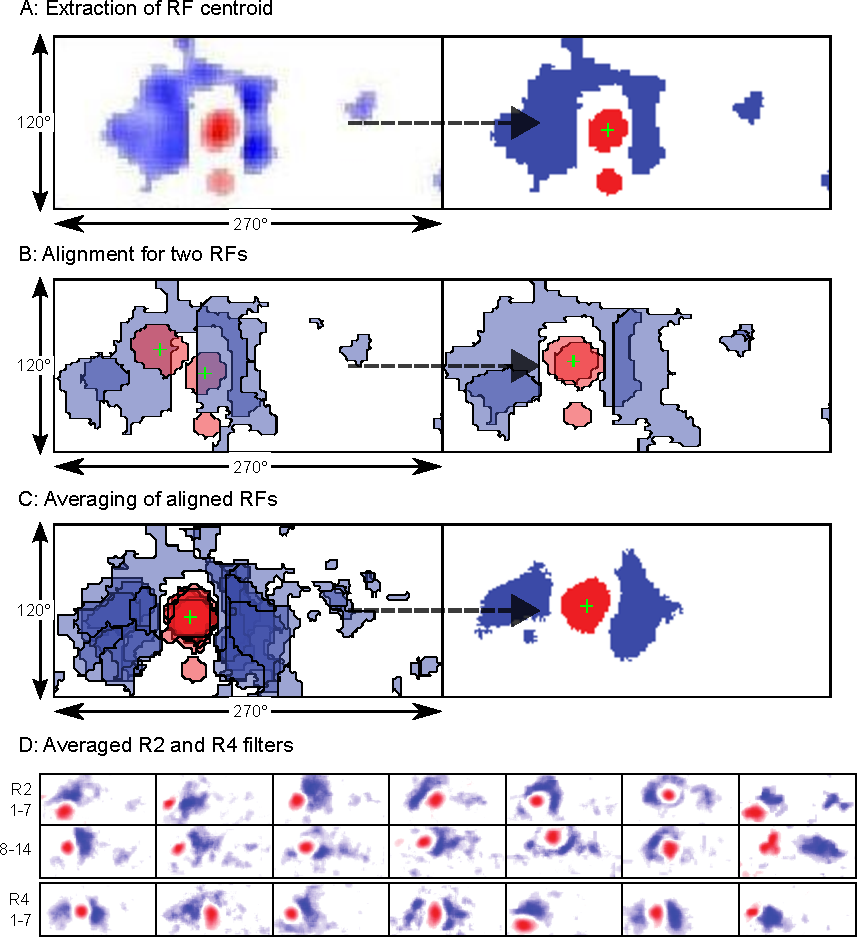
\includegraphics{figures/avkernels}
\caption{The algorithm for obtaining average RFs.}{
A: The raw image (left) is thresholded so as to give excitatory and inhibitory regions of uniform intensity (right).
The `centre' is then calculated as the centroid of the largest excitatory region (+).
B: Aligning two RFs.
The new centre is taken as the average of the centre of both RFs and the RFs are then shifted so that the centres are aligned.
C: Averaging the RFs for this glomerulus over all flies ($N=7$), following alignment.
Note that this the left-hemispheric version; the right-hemispheric version is its mirror.
Data are all for R4d glomerulus 1 neurons.}
\label{fig:avkernels}
\end{figure}


\subsection{Replication of behavioural experiments}
\label{sec:methods:replication}
The equation for describing the bar fixation mechanism shown in Figure~\ref{fig:recap}C is as follows:
$$
\phi_\mathrm{turn} = \frac{\mathrm{gain}\cdot \pi}{4}\left( \sum\limits_{K\in \mathbf{G}_\mathrm{left}}\max(0,A(I,K,0\degree)) - \sum\limits_{K\in \mathbf{G}_\mathrm{right}}\max(0,A(I,K,0\degree)) \right)
$$
where $I$ is the view of the bar from the agent's current location and $\mathbf{G}_\mathrm{left}$ and $\mathbf{G}_\mathrm{right}$ are the sets of left- and right-hemispheric filters. `Gain' is a parameter to control the gain of the system, and here was set to 2.

For the pattern recognition tasks (see Figure~\ref{fig:pattern}), the difference in activation is calculated as follows:
$$
D(I) = \sqrt{\frac{\sum\limits_{K\in \mathbf{G}}(A(I,K,0\degree)-A(I,K,90\degree))^2}{|\mathbf{G}|}}
$$
where $\mathbf{G}$ is the set of R2 filters, $I$ is the current pattern pair and $A(\cdot,\cdot,\cdot)$ is the activation of the kernel to the pattern, as described in Equation~\ref{eq:act}.

\subsection{Neural networks}
\label{sec:methods:neuralnetworks}
The neural networks were executed using the \texttt{Netlab} toolbox for \Matlab.
All networks were two-layer feedforward networks, with 10 hidden units and a linear activation function for the output units.
There were 100 training cycles and optimisation was performed with the scaled conjugate gradient method.

\subsubsection{Stimuli}
\label{sec:methods:stimuli}
The stimuli used to train the networks were trained were a series of black `blobs' on a white background.
The blobs were based on ellipses with a fixed ratio between the lengths of the major and minor axes ($2:1$), with the radii modified with complex waves:
$$
r(\theta) \le \left(\frac{\cos^2 \theta}{2} + \frac{\sin^2 \theta}{a} \right)^{-1} + W(\theta), \theta \in \{0, 2\pi\}
$$
where $a$ is the length of the major axis and $W(\theta)$ is a complex wave defined as:
$$
W(\theta) = \sum_{i=1}^n W_i(\theta) = \sum_{i=1}^n A_i \sin f_i (\theta+\phi_i) 
$$
where $A_i$, $f_i$ and $\phi_i$ describe the maximum amplitude, frequency and phase shift of the wave $W_i(\theta)$, respectively.
This method for generating stimuli allows for a substantial degree of random variation between the stimuli, while not producing shapes that are so irregular as to be unlearnable by a neural network.\todo{insertion}

In these experiments, $A_i$, $f_i$ and $\phi_i$ were randomly generated and $n=2$.
$A_i$ was a random value from 0 to 1, $f_i$ were random integers from 1 to 30 and $\phi_i$ was a random value from 0 to $2\pi$.
\begin{comment}
        nvar = 1000;
        nwave = 2;
        maxfreq = 30;
        maxamp = 1;
\end{comment}

The blobs were first generated, according to the above equation, as an image of $120\times 270$ pixels.
For the `raw view' stimuli, these images were resized, using \Matlab's \texttt{imresize} function, to $2\times 14$ pixels, thus giving the same number of inputs as there are R2 filters ($n=28$).

\begin{comment}
\subsubsection*{Grading performance of neural networks}
The performance of neural networks was graded by calculating the \ac{rms} difference between the matrix of true values for the parameters with the network's output:
$$
E(\mathbf{y},\mathbf{t}) = \sqrt{\frac{\sum\limits_{i=1}^{n} (\mathbf{y}_i-\mathbf{t}_i)^2}{n}}
$$
where $E(\mathbf{y},\mathbf{t})$ is the mean error score, computed from the vector of outputs given by the network, $\mathbf{y}$, and the vector of true values, $\mathbf{t}$.
Hence, for a network that computed the values of all parameters accurately, a graph of the network's output \emph{vs.} the true values would give the line $y=x$ and an error score of 0 over the whole range of values.
\end{comment}
